\documentclass[a4paper, 10pt, final]{article}
\usepackage{bonde}

\def\mytitle{Signal and Image Processing 2010}
\def\mysubtitle{Handin of mandatory excercise 1}
\def\myauthor{Ulrik Bonde}
\def\mymail{\mailto{bonde@diku.dk}}
\def\mydate{\today}

\title{\mytitle}
\subtitle{\mysubtitle}

\author{\myauthor{} - \mymail}
\date{\mydate}

\hypersetup{
colorlinks,%
citecolor=black,%
filecolor=black,%
linkcolor=black,%
urlcolor=black,%
bookmarksopen=false,
pdftitle={\mytitle{} - \mysubtitle},
pdfauthor={\myauthor}
}

\begin{document}
\maketitle

\subsection*{Question 1.1}
We wish to prove that the Fourier transform of a real and even function
is real and even. We solve the integral for the Fourier transform in
equation (2.18) \citet[p. 44]{jahne-digital}.

We split the integral in positive and negative parts, flip the
boundaries of the integral and perform the substitution $x = -x$.
\begin{align*}
    \hat{g}(k) & = \int_{-\infty}^{0}{g(x)\exp(-2\pi ikx)dx} + \int_{0}^{\infty}{g(x)\exp(-2\pi ikx)dx}\\
               & = \int_{0}^{\infty}{g(x)\exp(-2\pi ikx)dx} - \int_{0}^{-\infty}{g(x)\exp(-2\pi ikx)dx}\\
               & = \int_{0}^{\infty}{g(x)\exp(-2\pi ikx)dx} + \int_{0}^{\infty}{g(-x)\exp(2\pi ikx)dx}
\end{align*}

We use that $g(x) = g(-x)$ as we know that $g(x)$ is even and we can now
integrate from $0$ to $\infty$.
\begin{align*}
    \hspace{0.5em} &= \int_{0}^{\infty}{g(x)\exp(-2\pi ikx)dx} + \int_{0}^{\infty}{g(x)\exp(2\pi ikx)dx}\\
               & = \int_{0}^{\infty}{g(x)\left(\exp(-2\pi ikx) + \exp(2\pi ikx)\right)dx}
\end{align*}

By \emph{Euler's identities} we have that $\cos(\theta) =
\frac{e^{i\theta} + e^{-i\theta}}{2}$. We set $\theta = 2\pi kx$ and
multiply by $2$.
\begin{align*}
    \hspace{0.5em} & = 2 \int_{0}^{\infty}{g(x)\frac{\exp(-2\pi ikx) + \exp(2\pi ikx)}{2}dx}\\
               & = 2 \int_{0}^{\infty}{g(x)\cos(2\pi kx)dx}
\end{align*}

In the resulting $\hat{g}(k) = 2 \int_{0}^{\infty}{g(x)\cos(2\pi kx)dx}$
we have removed the imaginary part. The result is real and even because
$\cos(x)$ is an even function.

\subsection*{Question 1.2}
First we would like to find the Fourier transform of $\delta_{x - x_0} +
\delta_{x + x_0}$ (using the notation from \citeauthor{jahne-digital} for
$\delta$-functions). We set $g(x) = \delta_{x - x_0} + \delta_{x + x_0}$
and use equation (2.18) from \citeauthor{jahne-digital}.
\begin{align*}
    \hat{g}(k) & = \int_{-\infty}^{\infty}{g(x)\exp(-2\pi ikx)dx}\\
    & = \int_{-\infty}^{\infty}{(\delta_{x - x_0} + \delta_{x + x_0})e^{-2\pi ikx}dx}\\
    & = \int_{-\infty}^{\infty}{\delta_{x - x_0}e^{-2\pi ikx}dx +
    \int_{-\infty}^{\infty}{\delta_{-x - x_0}e^{-2\pi ikx}dx}}\\
\end{align*}

Note that we have used that $x + x_0 = -x - x_0$. In the second integral
we want to substitute $-x$ with $x$ to change signs in the exponential
function. To do this we have to multiply by $-1$ which changes the sign
of the integral. Also, the boundaries are reversed. We fix this by
changing the sign once again.
\begin{align*}
    & = \int_{-\infty}^{\infty}{\delta_{x - x_0}e^{-2\pi ikx}dx - \int_{\infty}^{-\infty}{\delta_{x - x_0}e^{2\pi ikx}dx}}\\
    & = \int_{-\infty}^{\infty}{\delta_{x - x_0}e^{-2\pi ikx}dx + \int_{-\infty}^{\infty}{\delta_{x - x_0}e^{2\pi ikx}dx}}
\end{align*}

When we integrate from $-\infty$ to $\infty$ there is only one point
where $x = x_0$ which means that the exponential functions in the
integral only contribute once. We then have that
\begin{align*}
    & = e^{-2\pi ikx} + e^{2\pi ikx}\\
    & = 2 \left(\frac{e^{-2\pi ikx} + e^{2\pi ikx}}{2}\right)\\
    & = 2 \cos(2\pi kx)
\end{align*}

By equation (2.19) from \citeauthor{jahne-digital} we have that
\begin{align*}
    g(x) & = \int_{-\infty}^{\infty}{\hat{g}(k)e^{2\pi ikx}dk}
\end{align*}
which will return the original function given the Fourier transform of
$g(x)$.

Based on the above we guess that the Fourier transform of $\cos(2\pi
xu_0)$ is $\frac{1}{2}(\delta_{x - x_0} + \delta_{x + x_0})$. We can
then do the inverse Fourier transform which should return the original
function.
\begin{align*}
    g(x) & = \int_{-\infty}^{\infty}{\frac{1}{2}(\delta_{x - x_0} +
    \delta_{x + x_0})e^{2\pi iu_0x}du_0}\\
    & = \frac{1}{2}\left( \int_{-\infty}^{\infty}{\delta_{x -
    x_0}e^{2\pi iu_0x}du_0} + \int_{-\infty}^{\infty}{\delta_{x +
    x_0}e^{2\pi iu_0x}du_0}\right)\\
    & = \cos(2\pi xu_0)
\end{align*}

We derive the result in a similar manner as previously except we
perform the substitution $u_0 = - u_0$. We use that the second
$\delta$-function can be written as $\delta_{x - (-x_0)}$ which then
again only contributes once.

\subsection*{Question 1.3}
The frequency of bass signals are low while treble signals have high
frequency.

\subsection*{Question 1.4}
Two MATLAB programs have been written. The program provide methods for
reducing the number of colors used to display an image and changing the
resolution of an image.

\subsubsection*{Reducing the number of colors}
\begin{figure}[!h]
    \centering
    \subfloat[Original]{\label{dark_original}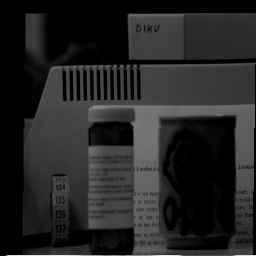
\includegraphics[angle=0,width=0.33\textwidth]{images/idotyl}\hspace{1em}}
    \subfloat[Histogram]{\label{darkhist}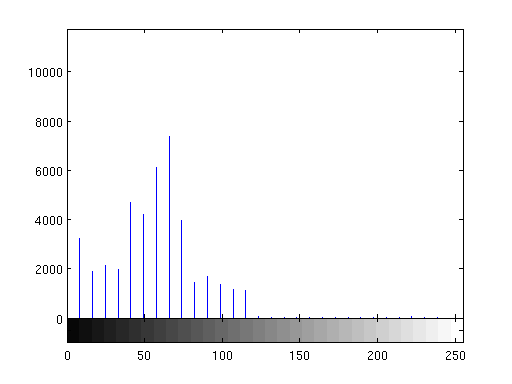
\includegraphics[angle=0,width=0.45\textwidth]{images/darkhist}}
    \caption[]{An image with its corresponding histogram. The histogram
    have been divided into 32 colors. Notice that the color values are
    not distributed on the entire set $(1,2\dots 255)$ and the image is
    very dark.}
    \label{dark_image}
\end{figure}

The approach used for reducing the number of colors in an image is very
similar to an image histogram. Such a histogram can be been in figure
\ref{dark_image}. Using the variable $n$ we can specify how many colors
we want. The color range is divided into $n$ smaller ranges of $255/n$
length. The subranges functions as bins where color values are put when
we scan an image. Pixel that belong to a certain bin will all be set to
the same value, which is the average of the boundaries of the bin.

If $n = 3$ we have three bins width a width of $255/3 = 85$. We have the
bins $\left[0; 85\right[$, $\left[85; 170\right[$ and $\left[170,
255\right]$.  The values given to pixel inside a bin is $42$, $127$ and
$212$ respectively.

We assume that the image have values ranging from $0$ to $255$. If
$n=3$ this causes problems with the image given in shown in figure
\ref{dark_image} as no pixel are found in the last bin and only two
colors will be used. This is illustrated in figure \ref{noadjust}.

\begin{figure}[!h]
    \centering
    \subfloat[No adjustment of colors]{\label{noadjust}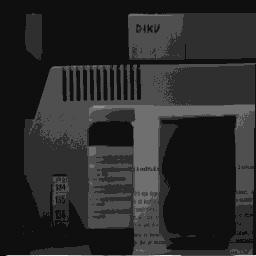
\includegraphics[angle=0,width=0.33\textwidth]{images/noadjust_8}\hspace{1em}}
    \subfloat[Colors adjusted]{\label{adjust}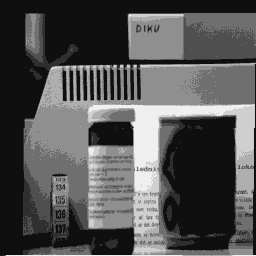
\includegraphics[angle=0,width=0.33\textwidth]{images/adjust_8}}
    \caption[]{The image from figure \ref{dark_image} shown with 8
    colors. The left image have not been adjusted and is very dark.
    Less than eight colors are used to shown the image. The right image
    have had its colors adjusted to fill out the entire range. Eight
    colors are used to show this image.}
    \label{n8}
\end{figure}

To avoid this behaviour it is best to adjust the colors of the image
before reducing the number of colors. This program adjust the each pixel
in the following manner.
\begin{equation*}
    I_{m, n} =  (I_{m, n} - I_{min})\frac{R_{max} - R_{min}}{I_{max} - I_{min}} + R_{min}
\end{equation*}
Here $R_{min}$ and $R_{max}$ are the interval which we wish to scale to
and $I_{min}$ and $R_{max}$ are the minimum and maximum values in the
original image. In practice the min and max values might not be
representative for the image. We use a 95 \% confidence interval for the
values for min and max.

The method always selects the average of the corresponding bin's
boundaries for the color. When $n$ is low these colors might not be
representative for the image, even though the colors have been adjusted.
A possible solution would be to find the actual mean of the colors in
the respective bins, thus selecting a more suitable shade for a given
pixel. In figure \ref{cr4} we might get a better shade for the computer
tower which were more related to the actual color in figure
\ref{cadjust}. Figure \ref{sequence_colors} shows when $n$ increases we
approximate the original colors.

\begin{figure}[!h]
    \centering
    \subfloat[No adjustment of colors]{\label{cnoadjust}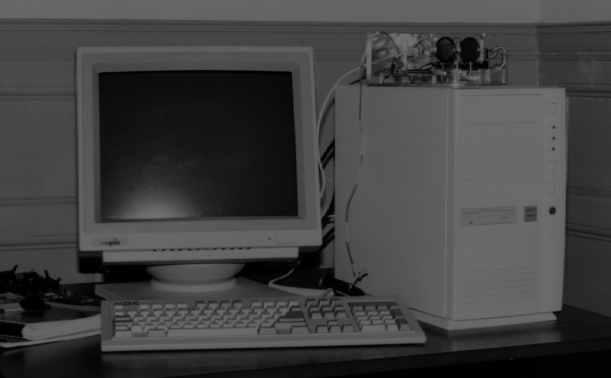
\includegraphics[angle=0,width=0.40\textwidth]{images/cNoAdjust}\hspace{1em}}
    \subfloat[Colors adjusted]{\label{cadjust}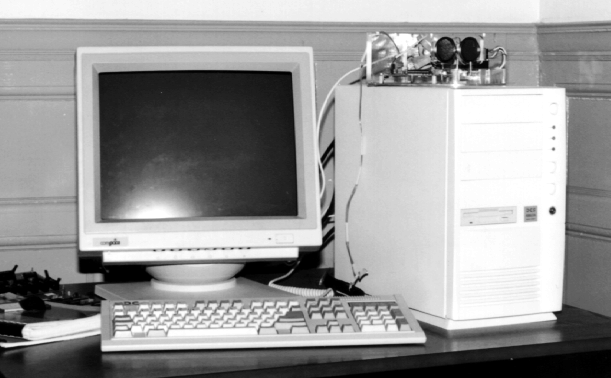
\includegraphics[angle=0,width=0.40\textwidth]{images/cAdjust}}\\
    \subfloat[$n = 4$]{\label{cr4}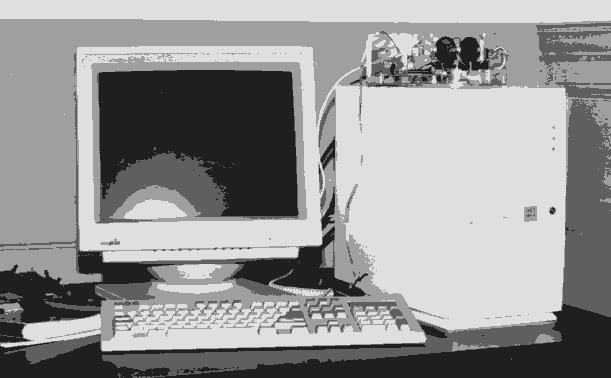
\includegraphics[angle=0,width=0.40\textwidth]{images/cr4}\hspace{1em}}
    \subfloat[$n = 8$]{\label{cr8}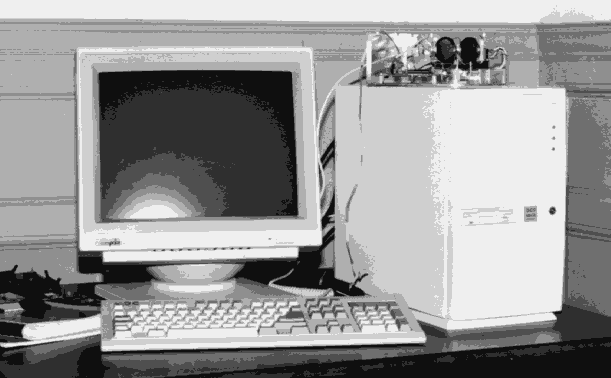
\includegraphics[angle=0,width=0.40\textwidth]{images/cr8}}\\
    \subfloat[$n = 16$]{\label{cr16}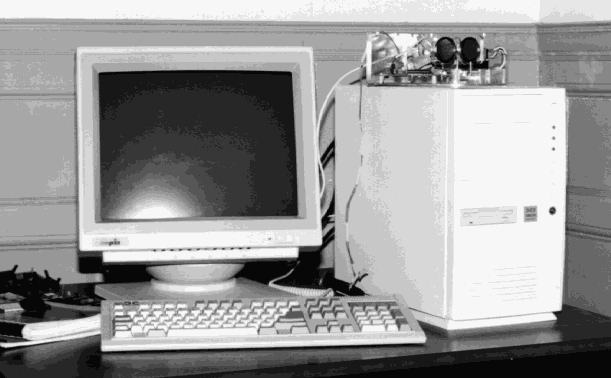
\includegraphics[angle=0,width=0.40\textwidth]{images/cr16}\hspace{1em}}
    \subfloat[$n = 32$]{\label{cr32}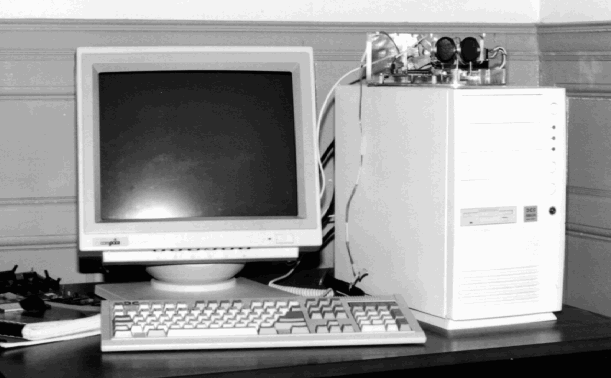
\includegraphics[angle=0,width=0.40\textwidth]{images/cr32}}\\
    \caption[]{A sequence of increasing colors to show the same image.
    The two top images show the original image before and after the
    colors have been adjusted. We gradually increase the number of
    colors from $4$ to $32$. Note the computer screen where the
    reflection shows a gradient from one extreme to another. With 16
    colors everything but the screen looks somewhat like the original.
    At 32 colors we almost have the same image as the original.}
    \label{sequence_colors}
\end{figure}

\subsubsection*{Changing the resolution}
To change the resolution in an image we use an integer $n$ to denote the
size of a $n \times n$ matrix used for subsampling a group of pixels. In
a smaller image, one pixel will represent a group of pixels in the
original. The image is then divided in to these groups of pixels as
shown in figure \ref{lenagrid}. The average value of this group of
pixels is then given to each pixel in the group.

\begin{figure}[!h]
    \centering
    \subfloat[Image with superimposed oversized pixels and $3\times3$
    matrices for subsampling]{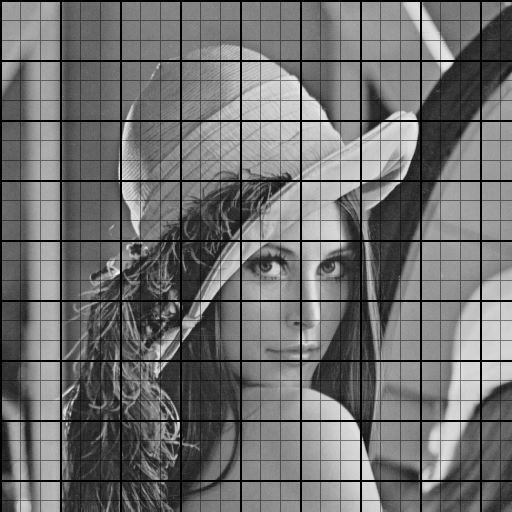
\includegraphics[scale=0.3]{images/Lena_grid}}\hspace{1em}
    \subfloat[Scaled image (zoomed in)]{
\includegraphics[scale=0.3]{images/LenaPixel}}
    \caption{In the left image the smaller lines indicate pixel borders. All
    pixels inside the subsampling matrix will be given the average
    value. Note that the matrix size is not a multiple of the image
    size. To the right, the rescaling have been performed. Note that the
    image dimensions have changed to include the pixels which could not
    fit.}
    \label{lenagrid}
\end{figure}


%%%%%%%%%%%%%%%%%%%%%%%%%%%%%%%%%%%%%%%%%%%%%%%%%%%%%%%%%%%%%%%%%%%%
% Formal stuff

\bibliographystyle{abbrvnat}
\bibliography{bibliography}
%\addcontentsline{toc}{chapter}{Litteratur}

\end{document}

% vim: set tw=72 spell spelllang=en:
